% ACCESS-NRI poster, converted from "ACCESS-NRI Poster template V4.pptx".
% Compile with XeLaTeX or LuaLaTeX:  xelatex poster.tex
%
% All positions below are in the PowerPoint template's own units (mm on a
% 395.1 x 558.4 mm slide) and are multiplied by \pscale. \pscale = 2.12851
% gives A0 (841 x 1189 mm); set it to 1 for the template's native size.
\documentclass{article}
\def\pscale{2.12851}

\usepackage{lmodern}
\usepackage{fontspec}
\usepackage{xcolor}
\usepackage{graphicx}
\usepackage{tikz}
\usepackage{amsmath}
\usepackage{enumitem}
\usepackage{url}
\urlstyle{same}

% ---------------------------------------------------------------- page
\newlength\pw \setlength\pw{395.111mm}\setlength\pw{\pscale\pw}
\newlength\ph \setlength\ph{558.447mm}\setlength\ph{\pscale\ph}
\newcommand\tl[1]{\dimexpr\pscale\dimexpr#1mm\relax\relax} % template mm -> page
\usepackage{geometry}
\geometry{paperwidth=\pw, paperheight=\ph, left=\tl{19.75}, top=\tl{128.4},
          right=\tl{19.75}, bottom=\tl{73}, noheadfoot}
\pagestyle{empty}
\setlength\parindent{0pt}
\frenchspacing

% ---------------------------------------------------------------- fonts
% The template uses Arial and Arial Black. Fall back to Helvetica clones
% (Nimbus Sans on Linux, TeX Gyre Heros on Overleaf) when they're missing.
\def\urwpath{/usr/share/fonts/urw-base35/}
\IfFontExistsTF{Arial}{\setmainfont{Arial}}{%
  \IfFileExists{\urwpath NimbusSans-Regular.otf}{%
    \setmainfont{NimbusSans}[Path=\urwpath, Extension=.otf, UprightFont=*-Regular,
      BoldFont=*-Bold, ItalicFont=*-Italic, BoldItalicFont=*-BoldItalic]}{%
    \setmainfont{TeX Gyre Heros}}}
\IfFontExistsTF{Arial Black}{\newfontfamily\blackfont{Arial Black}}{%
  \newcommand\blackfont{\bfseries}}

\makeatletter
% \setfs{size}{baselineskip}, in template pt (scaled by \pscale)
\newcommand\setfs[2]{%
  \edef\@fsa{\strip@pt\dimexpr\pscale\dimexpr#1pt\relax\relax}%
  \edef\@fsb{\strip@pt\dimexpr\pscale\dimexpr#2pt\relax\relax}%
  \fontsize{\@fsa}{\@fsb}\selectfont
  \spaceskip=0pt \xspaceskip=0pt}% TikZ's align= fixes these at the node's start-up size
\makeatother

% ---------------------------------------------------------------- colours
\definecolor{nriblue}{HTML}{236298}  % header / website
\definecolor{nricyan}{HTML}{00ADEE}  % colour bar
\definecolor{nrisky}{HTML}{8DD7F7}
\definecolor{nrinavy}{HTML}{005B94}
\definecolor{nrigreen}{HTML}{A5CD39}

% ---------------------------------------------------------------- content macros
\newlength\colw  \setlength\colw{\tl{111.87}}
\newlength\colgap \setlength\colgap{\tl{10}}

\newcommand\posterhead[2][]{% [number]{heading}
  \par\vspace{\tl{6}}%
  {\blackfont\setfs{22}{26}\color{nriblue}%
   \ifx\relax#1\relax\else#1\enspace\fi#2\par}\vspace{\tl{2.5}}}

% \firstin{experiment}: first 25 km IAF experiment with the change, under a heading
\newcommand\firstin[1]{\firstinline{First in: #1}}
\newcommand\firstinline[1]{\vspace{-\tl{1}}{\setfs{11}{13}\color{black!60}#1\par}%
  \vspace{\tl{2}}}

% \posterfig[width]{file}{caption}
\newcommand\posterfig[3][\linewidth]{%
  \par\vspace{\tl{3}}{\centering\includegraphics[width=#1]{#2}\par}%
  \vspace{\tl{1.2}}{\setfs{10}{12}\color{black!70}#3\par}\vspace{\tl{2}}}

% \placeholderfig{height mm}{what goes here}
\newcommand\placeholderfig[2]{%
  \par\vspace{\tl{3}}\noindent
  \tikz\node[draw=nriblue, dashed, line width=\tl{0.4}, fill=nrisky!20,
             minimum width=\linewidth-\tl{0.4}, minimum height=\tl{#1},
             text width=0.85\linewidth, align=center, inner sep=0pt,
             font=\setfs{12}{14}, text=nriblue]
            {FIGURE TO ADD\\[0.3em]#2};%
  \par\vspace{\tl{2}}}

\setlist{leftmargin=1.1em, itemsep=0.15em, topsep=0.2em, parsep=0pt}
\setlist[itemize]{label=\textcolor{nricyan}{\textbullet}}

% ---------------------------------------------------------------- poster text
\newcommand\headline{Tip of the\\(melted) iceberg}
\newcommand\postertitle{Freshwater Forcings in ACCESS-OM3}
\newcommand\posterauthors{Anton Steketee\textsuperscript{1}, Andrew Kiss\textsuperscript{2},
  Dougie Squire\textsuperscript{1}, Ezhil Kannadasan\textsuperscript{1}}
\newcommand\posteraffils{\textsuperscript{1}Australia's Climate Simulator (ACCESS-NRI),
  Australian National University, Canberra, Australia\\
  \textsuperscript{2}Research School of Earth Sciences, Australian National University,
  Canberra, Australia}

\begin{document}
% ================================================================ template frame
\begin{tikzpicture}[remember picture, overlay, x=\pscale mm, y=-\pscale mm,
                    shift={(current page.north west)}]
  % blue header band
  \fill[nriblue] (0,0) rectangle (395.111,74.56);
  % white cut-out behind the ACCESS logo (ellipse fitted to the template's traced path)
  \begin{scope}
    \clip (0,0) rectangle (395.111,558.447);
    \fill[white] (352.08,35.09) ellipse [x radius=67.49, y radius=63.85];
  \end{scope}
  \node[anchor=north west, inner sep=0] at (284.59,11.69)
    {
\includegraphics[width=\tl{105.38}]{logos/access.png}};
  \node[anchor=north west, inner sep=0, text=nriblue, font=\setfs{21}{24}\bfseries]
    at (308.23,57.20) {access-nri.org.au};

  % plain-English summary of the main findings (white, in the header)
  \node[anchor=north west, inner sep=0, text=white, text width=\tl{222}, align=left,
        font=\blackfont\setfs{51}{71}] at (15.69,13.6) {\headline};

  % title and authors
  \node[anchor=north west, inner sep=0, text width=\tl{265}, align=left,
        font=\setfs{20}{24}] at (15.69,86.5)
    {{\blackfont\setfs{36}{42}\postertitle\par}\vspace{\tl{3}}%
     {\setfs{20}{24}\posterauthors\par}\vspace{\tl{1.5}}%
     {\setfs{13}{16}\color{black!70}\posteraffils\par}};

  % AI declaration (bottom left, clear of the partner logos)
  \node[anchor=north west, inner sep=0, text width=\tl{120}, align=left,
        font=\setfs{9}{11}, text=black!60] at (19.75,492)
    {\textbf{AI declaration:} Claude (Anthropic) assisted with poster
     preparation and parts of the software development. All content was
     reviewed by the authors.};

  % footer: colour bar, partner logos, NCRIS
  \node[anchor=north west, inner sep=0] at (87.75,488.16)
    {
\includegraphics[width=\tl{307.2}, height=\tl{10.94}]{logos/colourbar.png}};
  \node[anchor=north west, inner sep=0] at (74.86,515.99)
    {
\includegraphics[width=\tl{207.53}, height=\tl{16.49}]{logos/partners.jpg}};
  \node[anchor=north west, inner sep=0] at (314.62,502.75)
    {
\includegraphics[width=\tl{59.91}, height=\tl{43.31}]{logos/ncris.jpg}};
\end{tikzpicture}%
% ================================================================ body
\setfs{14}{17.5}%
% ---------------------------------------------------------------- column 1
\begin{minipage}[t]{\colw}\raggedright
\posterhead{Why?}
ACCESS-OM3 couples an interactive ocean and sea ice to a \emph{fixed}
atmosphere and runoff: the JRA55-do forcing, a reconstruction of past weather
and river flows built from observations and a weather model (Tsujino et al.\
2018).
\begin{itemize}
  \item model evaporation doesn't balance the prescribed rain and runoff
  \item runoff and iceberg melt land where the forcing grid puts them
\end{itemize}

\vspace{\tl{3}}
{\centering
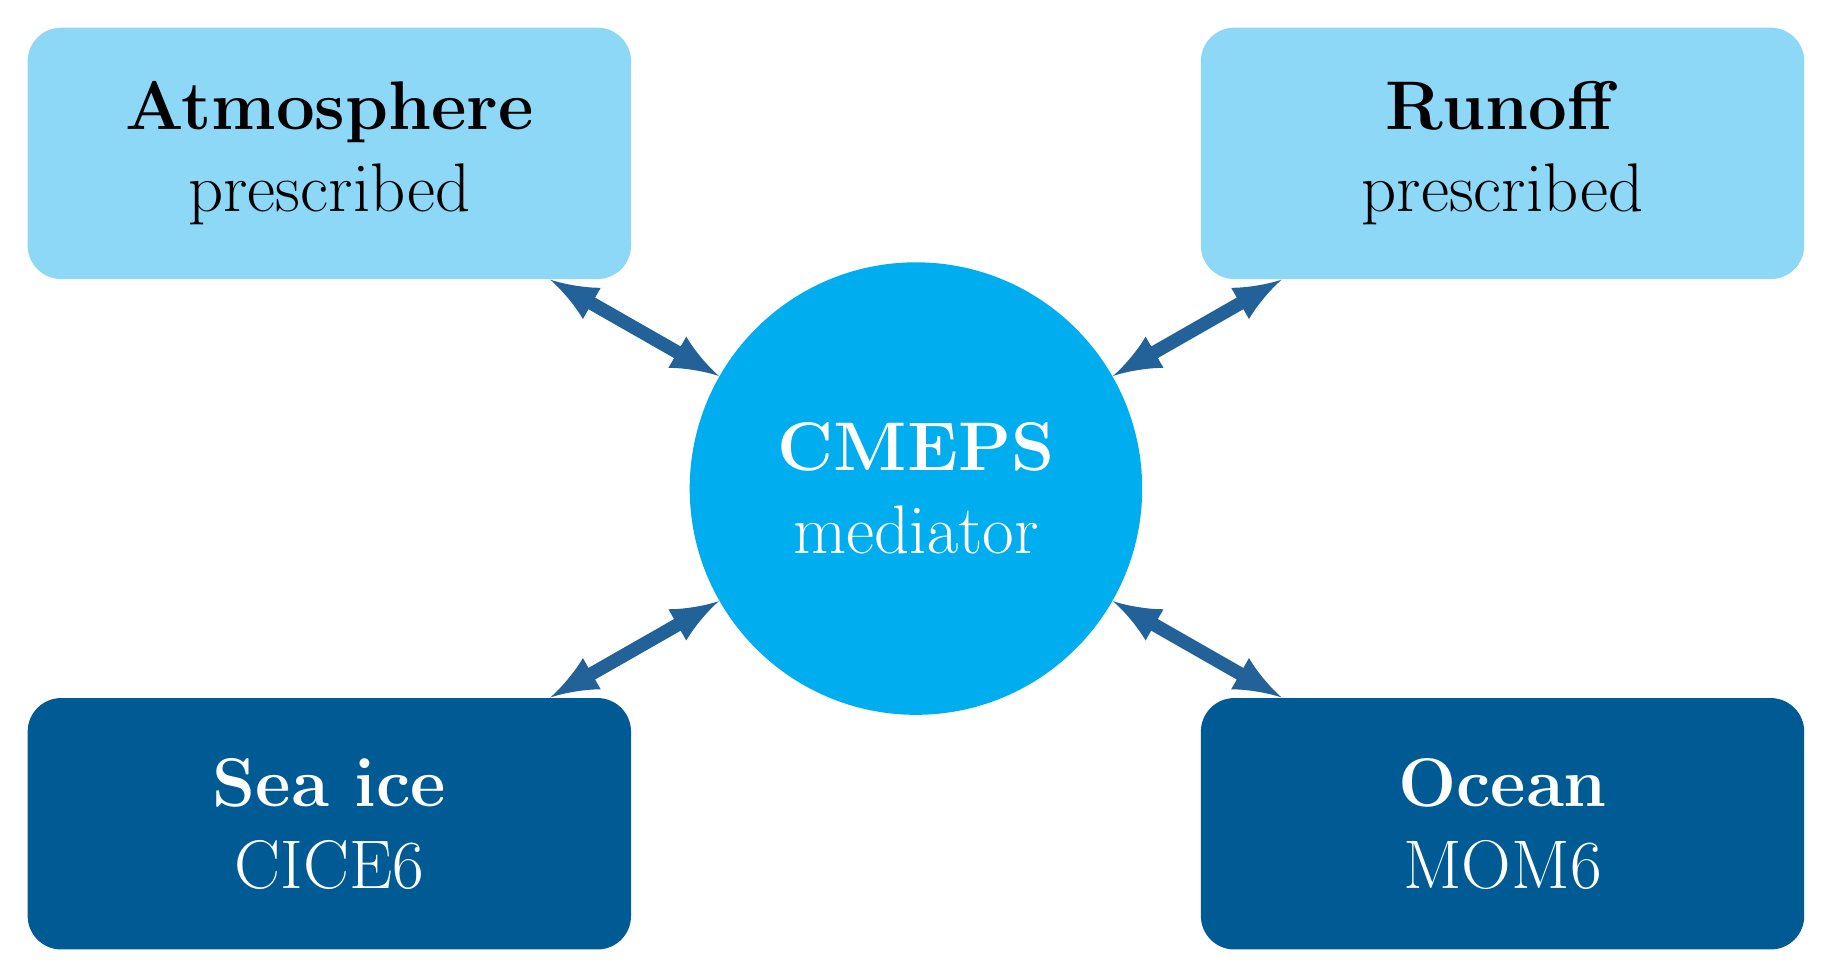
\begin{tikzpicture}[x=\pscale mm, y=\pscale mm, font=\setfs{12}{14},
    comp/.style={rounded corners=\tl{2}, minimum width=\tl{36}, minimum height=\tl{15},
                 align=center, inner sep=\tl{1}},
    data/.style={comp, fill=nrisky},
    live/.style={comp, fill=nrinavy, text=white},
    link/.style={<->, >=latex, line width=\tl{0.8}, nriblue}]
  \node[circle, fill=nricyan, text=white, minimum size=\tl{27}, align=center,
        inner sep=0] (med) at (0,0) {\textbf{CMEPS}\\mediator};
  \node[data] (atm) at (-35, 20) {\textbf{Atmosphere}\\prescribed};
  \node[data] (rof) at ( 35, 20) {\textbf{Runoff}\\prescribed};
  \node[live] (ice) at (-35,-20) {\textbf{Sea ice}\\CICE6};
  \node[live] (ocn) at ( 35,-20) {\textbf{Ocean}\\MOM6};
  \foreach \n in {atm,rof,ice,ocn} \draw[link] (\n) -- (med);
\end{tikzpicture}\par}
\vspace{\tl{1}}
{\setfs{10}{12}\color{black!70}Light boxes are read from the forcing; dark
boxes are interactive models. All fixes below live in the CMEPS mediator, the
only component that sees every flux.\par}

\posterhead[1]{Global freshwater balance}
\firstin{25\,km IAF test4; 8\,km RYF test2}
Each coupling step, precipitation $P$ is scaled so that runoff $R$ and
evaporation $E$ into ocean + sea ice sum to zero:
\[ sP + R + E = 0 \quad\Rightarrow\quad s = 1 - \frac{P+R+E}{P} \]
Unlike an offset, scaling can't create negative rain. This scaling accounts for water
held in sea ice and snow, unlike the base case.
\posterfig{figs/fw_mass_constant.png}{Total ocean + sea ice mass (bottom)
oscillates without the balance (base) and is constant with it (new).}

\vspace{\tl{6}}
{\setfs{10}{12}\color{black!70}\textbf{References}\par\vspace{\tl{1}}
Schmidt, G.\,A., Mankoff, K.\,D., Bamber, J.\,L., et al.\ (2025). Datasets and
protocols for including anomalous freshwater from melting ice sheets in climate
simulations. \emph{Geosci.\ Model Dev.}, 18, 8333.
\url{https://doi.org/10.5194/gmd-18-8333-2025}\par\vspace{\tl{1}}
Tsujino, H., et al.\ (2018). JRA-55 based surface dataset for driving
ocean--sea-ice models (JRA55-do). \emph{Ocean Modelling}, 130, 79--139.
\url{https://doi.org/10.1016/j.ocemod.2018.07.002}\par}
\end{minipage}\hspace{\colgap}%
% ---------------------------------------------------------------- column 2
\begin{minipage}[t]{\colw}\raggedright
\posterhead[2]{Spreading river runoff}
\firstin{25\,km IAF test5; 8\,km RYF test2}
\begin{minipage}[t]{0.45\linewidth}\vspace{0pt}
  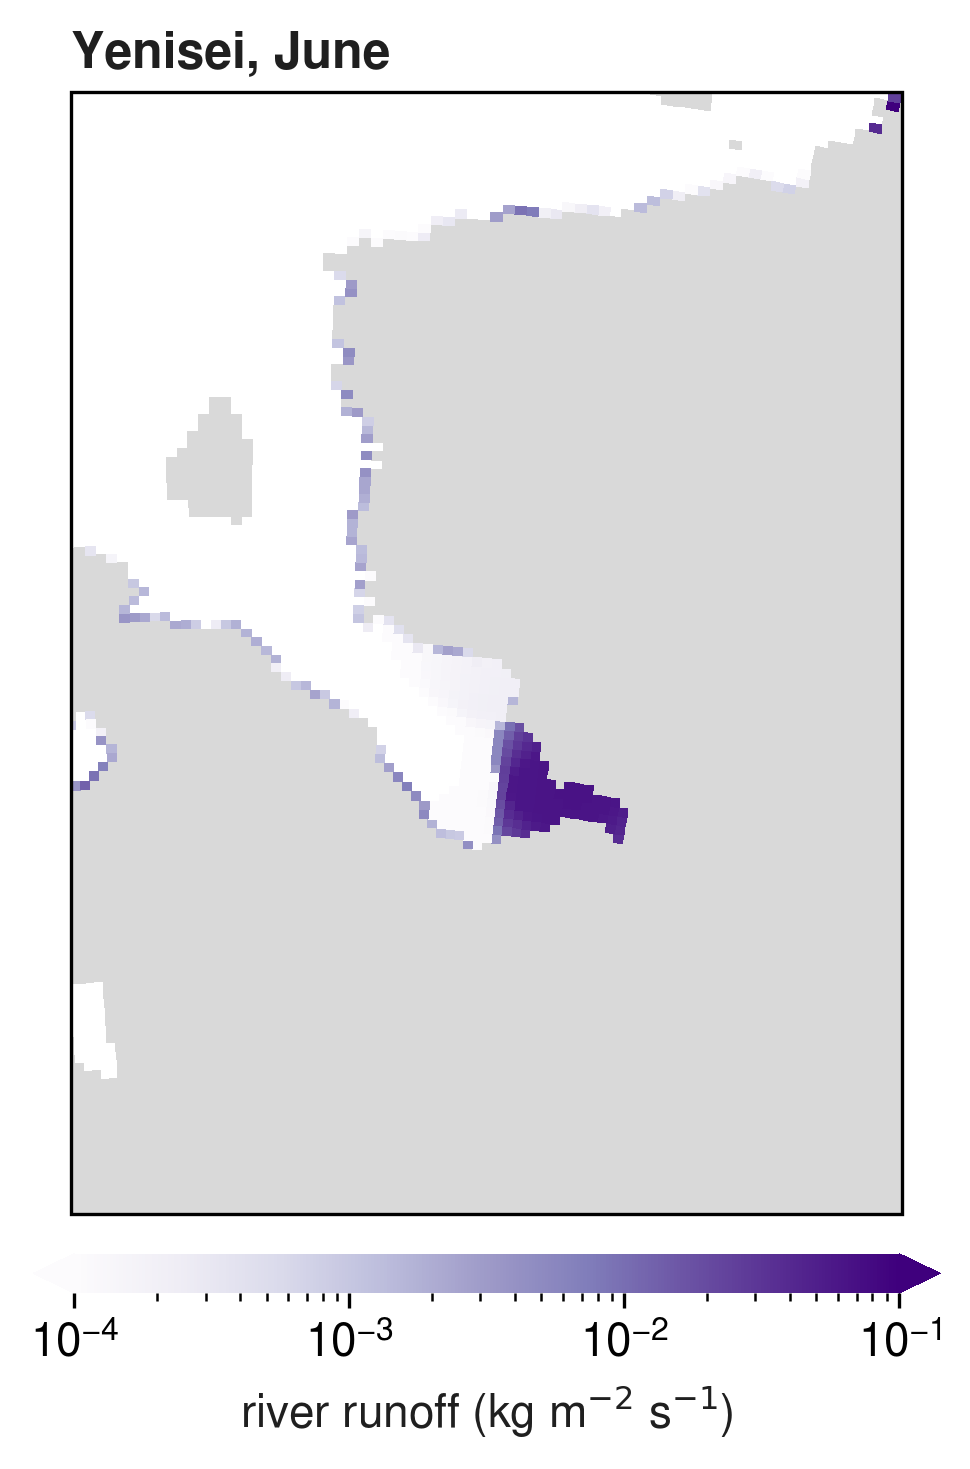
\includegraphics[width=\linewidth]{figs/river_yenisei_8km_test2.png}
\end{minipage}\hfill
\begin{minipage}[t]{0.52\linewidth}\vspace{0pt}\raggedright
  Large rivers (Amazon, Yenisey, Lena,~\dots) no longer pour into one coastal cell.
  Their runoff is:
  \begin{itemize}
    \item spread over the nearest 75 ocean cells
    \item weighted by distance ($e$-folding 2\textdegree)
    \item area-weighted, so volume is conserved
  \end{itemize}
\end{minipage}
\vspace{\tl{1.2}}
{\setfs{10}{12}\color{black!70}Yenisei runoff in June (8\,km test run), spread
from the head of the gulf over the nearby ocean.\par}

\posterhead[3]{Spreading iceberg melt}
\firstin{25\,km IAF test4; 8\,km RYF test2}
The forcing puts all iceberg melt on the coast. We spread it, and the latent heat
needed to melt it, offshore using a monthly climatology (Schmidt et al.\ 2025),
renormalised so no water is lost.
\posterfig{figs/rofi_jan_maps_scaled_spread.png}{Antarctic iceberg melt,
January 1958 (100\,km test): forcing input, after seasonal scaling, and after
spreading.}

\posterhead[4]{Seasonal iceberg melt}
\firstinline{Not yet in a shared experiment}
In the forcing, Antarctic iceberg melt is constant in time. Monthly factors from the
same climatology now give a summer peak (${\sim}2.6\times$ in Jan--Feb,
${\sim}0.3\times$ in Sep) with the annual total unchanged.
\posterfig{figs/rofi_seasonal_timeseries_sh.png}{Southern Hemisphere iceberg
melt: forcing input (dashed) and after scaling and spreading.}
\end{minipage}\hspace{\colgap}%
% ---------------------------------------------------------------- column 3
\begin{minipage}[t]{\colw}\raggedright
\posterhead[5]{Impacts}
\textbf{Latent heat:} melting icebergs takes heat from the ocean. With all the
melt on the coast, that heat came from a thin ring of coastal cells, freezing
spurious frazil ice there. Spreading more than halves coastal frazil.
\posterfig{figs/impact_frazil.png}{Frazil ice growth in 25\,km 1958--2023 runs
without (before) and with (after) these changes. Coastal cells: the first ocean
cell next to land.}

\textbf{Salinity restoring:} with each big river emptying into one cell, the
surface there got fresh enough to crash the CICE sea ice thermodynamics, which
only strong salinity restoring prevented. Spreading the runoff, in conjunction
with other changes, improves model stability by reducing the total area with
unrealistically low salinity, so a weaker restoring rate can be used (now being
tested).
\posterfig{figs/impact_fresh_area.png}{Area where monthly minimum surface
salinity is below 1 or 5\,psu, 25\,km test4 (before) and test5 (after: river
spreading plus other changes), 1958--1973.}

\posterhead{Ongoing work}
The forcing's liquid runoff south of 60\textdegree S is really ice-shelf basal
melt. We are splitting it into its own field so that it can:
\begin{itemize}
  \item take the latent heat needed to melt the ice from the ocean
  \item enter the ocean at depth
\end{itemize}

\vspace{\tl{4}}
\noindent\colorbox{nrisky!35}{\begin{minipage}{\dimexpr\linewidth-2\fboxsep\relax}\raggedright
\vspace{\tl{2}}
{\blackfont\setfs{18}{22}\color{nriblue}Take-home\par}\vspace{\tl{1.5}}
\begin{itemize}
  \item Ocean + sea ice fresh water is globally balanced
  \item Rivers and icebergs deliver fresh water, and its heat, where it belongs
  \item Antarctic iceberg melt has a realistic seasonal cycle
\end{itemize}
\vspace{\tl{2}}
\end{minipage}}
\end{minipage}
\end{document}
